\documentclass{article}
\usepackage[utf8]{inputenc}
\usepackage{graphicx} % Required for including images

\title{Random Research Document}
\author{Generated Author}
\date{\today}

\begin{document}

\maketitle

\section{Introduction}
This document serves as a demonstration of a LaTeX file interacting with a BibTeX database. 

\begin{figure}[h]
    \centering
    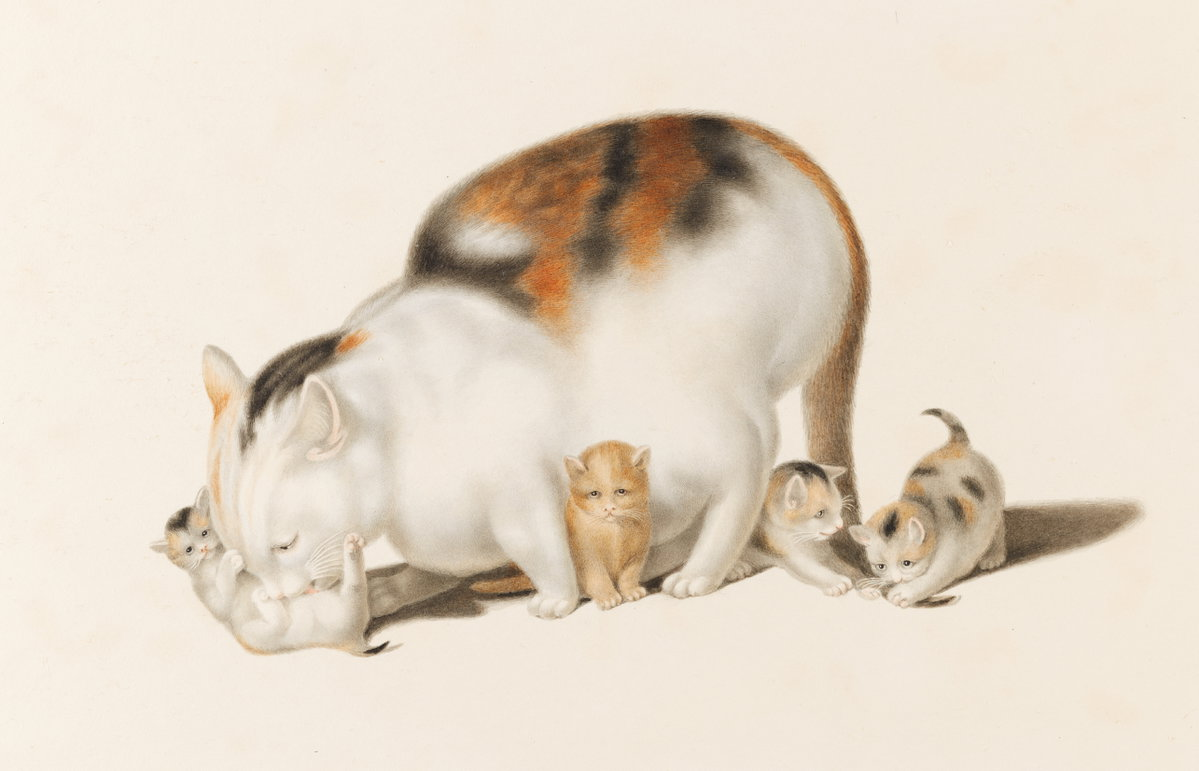
\includegraphics[width=0.5\textwidth]{assets/cat.jpg}
    \caption{A demonstration of an included image.}
    \label{fig:cat}
\end{figure}

\section{Literature Review}
In the field of quantum studies, several authors have made significant contributions. 
For instance, the work in \cite{ref1} and \cite{ref2} laid the groundwork. 
Subsequent studies by \cite{ref3}, \cite{ref4}, and \cite{ref5} expanded on these theories.
Additional context can be found in the following references: \cite{ref6}, \cite{ref7}, \cite{ref8}, \cite{ref9}, and \cite{ref10}.

To reach our target of 26 referred entries, we cite six more unique entries:
The methodologies described in \cite{ref11} and \cite{ref12} are particularly relevant. 
Furthermore, \cite{ref13}, \cite{ref14}, \cite{ref15}, and \cite{ref16} provide the necessary data for our analysis.

\section{Conclusion}
The remaining 24 entries in the bibliography are not cited in this text.

\bibliographystyle{plain}
\bibliography{references}

\end{document}